\chapter{DoA Estimation: Super-resolution via MuSiC}
\label{ch:OverviewMUSIC}

\section{Introduction}
The \gls{music} algorithm is a prominent high-resolution method in the realm of \gls{doa} estimation.
This chapter offers a brief overview of its fundamental mathematical underpinnings and practical considerations,
particularly highlighting the essentiality of prior knowledge of the model order \( N \). Although, a manifold of
variations of \gls{music} exist, this chapter focuses exclusively on the original \gls{music} algorithm, since these
variations still require \( N \) to be known a priori.

As hinted in the introductory chapter, super-resolution methods, including \gls{music}, differ significantly from
conventional \gls{doa} estimation methods. It was previously mentioned that conventional techniques like correlation
interferometers and beam-formers, while computationally efficient, fail to handle multiple incoming waves within a single
frequency bin. Super-resolution methods, on the other hand, are capable of estimating the \gls{doa} of signals even when
their angular separation is less than the beam-width of the antenna array. This capability is often refferred to as
``super-resolution''~\cite{tuncer.ch1}.

Theoretically, \gls{doa} estimation could be optimally achieved using a \glsdesc{mle} approach, as outlined
in~\cite{tuncer.ch1}. However, this method becomes computationally unsustainable for large antenna arrays, as it requires
an exhaustive search over an \( N \)-dimensional complex space.
In contrast, while the computational complexity of \gls{music} is higher compared to conventional methods, it remains
feasible for large arrays by reducing the search to a two-dimensional grid.
However, a notable limitation of \gls{music} is its requirement for a
higher number of snapshots \( K \), whereas conventional methods can already achieve reasonable results with a single
snapshot. This requirement for a higher number of snapshots is due to the need for a higher
\gls{snr} for accurate estimation~\cite{tuncer.ch1}.

\section{The MuSiC Algorithm}
\label{sec:music_algorithm}
The \gls{music} algorithm is predicated on the principles of subspace decomposition which were outlined in~\autoref{sec:CovarianceMatrix}.
It exploits the orthogonality between the signal subspace \( \UsH \) and the noise subspace \( \UnH \).
This perpendicularity is mathematically captured by the vanishing inner product between these two subspaces, as indicated
in~\autoref{eq:orthogonality}.

\begin{equation}
    \UsH^H \UnH = 0
    \label{eq:orthogonality}
\end{equation}

Building upon the concept that \( \UsH \) comprises a linear combination of the steering vectors \( (\bfm{a}(\bfT_1), \ldots, \bfm{a}(\bfT_N)) \),
as discussed in~\autoref{sec:sub:subspaces}, this orthogonality condition can be reformulated such that it becomes a
function of \( \bfT \).

\begin{equation}
    \bfm{a}^H(\bfT) \UnH = 0 \quad \text{for } \bfT \in \{\bfT_1, \ldots, \bfT_N\}
    \label{eq:orthogonality2}
\end{equation}

\autoref{eq:orthogonality2} underpins the formulation of the MuSiC pseudo-spectrum \( \widehat{P}_{\text{MuSiC}}(\bfT) \), defined as:
\begin{equation}
    \widehat{P}_{\text{MuSiC}}(\bfT) = \frac{1}{\|\bfm{a}^H(\bfT) \UnH \|^2}
\end{equation}

The MuSiC pseudospectrum is instrumental in identifying the \gls{doa} of incoming signals, as it exhibits local maxima
corresponding to the true \gls{doa} angles. In an ideal scenario without noise, the pseudo-spectrum would exhibit
infinite peaks at these angles. With the prerequisite knowledge of the model order \( N \), which signifies the number
of impinging waves, the task of estimating the \glspl{doa} translates into an optimization problem. The objective is to
locate the \( N \) angles \( \bfT \) that maximize the pseudo-spectrum. This optimization problem can be formally stated as:

\begin{equation}
    \{\widehat{\bfT}_1, \ldots, \widehat{\bfT}_N\} = \argmax_{\bfT} \widehat{P}_{\text{MuSiC}}(\bfT)
\end{equation}

\subsubsection*{Visualizing the MuSiC Pseudospectrum}
\autoref{fig:music_pseudospectrum} presents a three-dimensional conceptual plot of the pseudo-spectrum, delineated across
azimuth \( \azim \) and elevation \( \elev \) angles. The pronounced peaks, marked in red, correspond to the estimated
\glspl{doa} of the impinging signals. Notably, \( \bfT_3 \) and \( \bfT_4 \) display discernible deviations from the true
local maxima within the spectrum. Errors in the \gls{doa} estimates are usually quantified via the \gls{rmse} metric,
expressed in degrees.

\begin{figure}[H]
    \centering
    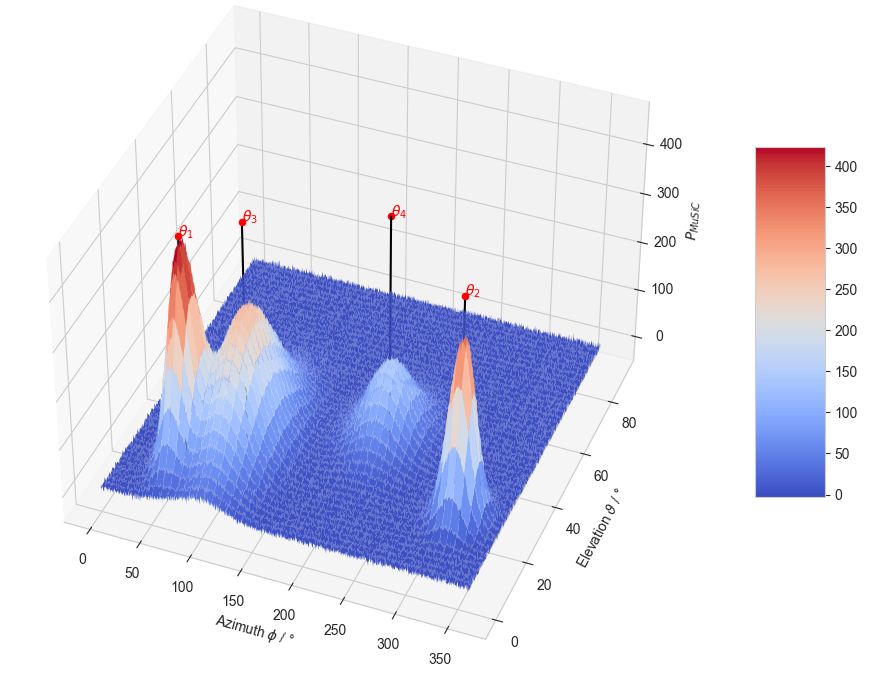
\includegraphics[width=0.76\textwidth]{figures/03_music/music_spectrum.png}
    \caption{Conceptual visualization of the MuSiC pseudo-spectrum for \( N = 4 \) impinging waves.}
    \label{fig:music_pseudospectrum}
\end{figure}

In practice, the accuracy of the peak detection directly influences the reliability of the \gls{doa} estimates.
Since the actual signal subspace \( \UsH \) is not utilized in computing the \gls{music}
spectrum, a peak's magnitude does not reflect signal strength. Instead, both the extent and magnitude of the peaks
are associated with the angular resolution and the adequacy of the estimated subspaces \( \UsH \) and \( \UnH \)
in representing the true subspaces. This can be attributed to a well approximated covariance matrix \(  K \gg 3M \implies \C \rightarrow \bfm{C}_x \),
a correct model order estimate \( \NPred = N \) a good fit of the estimated array manifold \( \mathfrak{A} \), which is heavily contingent on accurate calibration of the
antenna array.


\subsection{Summary of the MuSiC Algorithm}

\begin{figure}[H]
    \centering
    \includegraphics[width=1\textwidth]{figures/03_music/MuSiC.pdf}
    \caption{Block diagram / flowchart of the MuSiC algorithm.}
    \label{fig:music_algorithm}
\end{figure}

To succinctly summarize the MuSiC algorithm in accordance with \autoref{fig:music_algorithm}, we delineate the sequence
of its operational steps. Initially, the measurement vector \( \bfm{x} \) is captured to estimate the covariance
matrix \( \C \). Following this, the matrix undergoes eigenvalue decomposition to segregate the signal \( \UsH \) and
noise \( \UnH \) subspaces. The subsequent action is the estimation of
the model order \( \NPred \). This estimation can be achieved using methodologies such as \gls{aic}, \gls{mdl}, \gls{eft},
or neural networks and will be the focus of the remaining chapters.
With \( \NPred \) determined, an optimization approach, such as a grid search
\footnote{There are various optimization approaches and search-free variations of MuSiC.},
is employed to discern the \( \widehat{N} \) angles of arrival \( \{\widehat{\bfT}_1, \ldots, \widehat{\bfT}_{\NPred}\} \)
that elicit the peak responses from the MuSiC pseudo-spectrum \( \widehat{P}_{\text{MUSIC}}(\bfT) \).
The process concludes by calculating the MuSiC quality metrics as per \autoref{eq:music_quality}, which evaluate the accuracy of the \gls{doa}
estimates through the congruence of the steering vectors to the signal subspace. These procedural steps form the essence
of the MuSiC algorithm, cohesively represented in the accompanying flowchart.

\begin{equation}
    Q_{n}(\bfT_n) = \frac{\|\UsH^H\bfm{a}\left(\widehat{\bfT}\right)\|}{\|\bfm{a}^H\left(\widehat{\bfT}\right)\|}, \quad Q_n \in [0, 1], \quad n \in \{1, \ldots, \NPred\}
    \label{eq:music_quality}
\end{equation}

Another reason to define the \gls{music} quality metric in this thesis will become apparent in the last chapter
(\autoref{ch:conclusion_outlook}), where a variety of possible enhancements will be presented.

\endinput

